\chapter{Proposal for a Multi-agent Tournament System}
\label{appendix:aivle-web_matchmaking}

In the previous version of aiVLE 2.0, we already have infrastructure for running arbitrary evaluation as a Job instance. Here we propose an extension to support multi-agent on aiVLE (both matchmaking and evaluation).

This design is very high-level and abstract: even though all relevant code is concrete and runnable, the matchmaking algorithm/strategy, which happens to be the most important and sophisticated part of matchmaking, is not provided. On the other hand, this also means that our design is not limited to any specific tournament type or matchmaking algorithm.

\section{Tournament Abstraction}
\label{as:matchmaking-api_design-tournament_abstraction}
Before we dive into the actual API design, we need to understand what is common to all tournament. A tournament consists of one or many rounds of matches. The participants in every match of a certain round are determined before the round starts, and the order of matches within a round does not matter. After every round, we determine whether the tournament has concluded, or generate the match schedule for the next round.

Here we show the generality of such description by applying it to a real-world championship series: the Overwatch League (OWL)\footnote{The Overwatch League is a professional e-sports league for the video game Overwatch. Its structure and operation is similar to other American sports championships such as NBA (National Basketball Association).} championship:

OWL has regular season matches and playoffs. The schedule for regular season is determined before the season starts, and is not affected by the outcome of any matches within. So we may consider the entire regular season as one round.

The list of teams advanced to the playoffs is determined by the regular season results, so starting the playoffs also means starting a new round. Here we take regular season tournament format of OWL 2021 as an example (Figure~\ref{fig:owl-tournament-format}):

\begin{figure}[H]
    \centering
    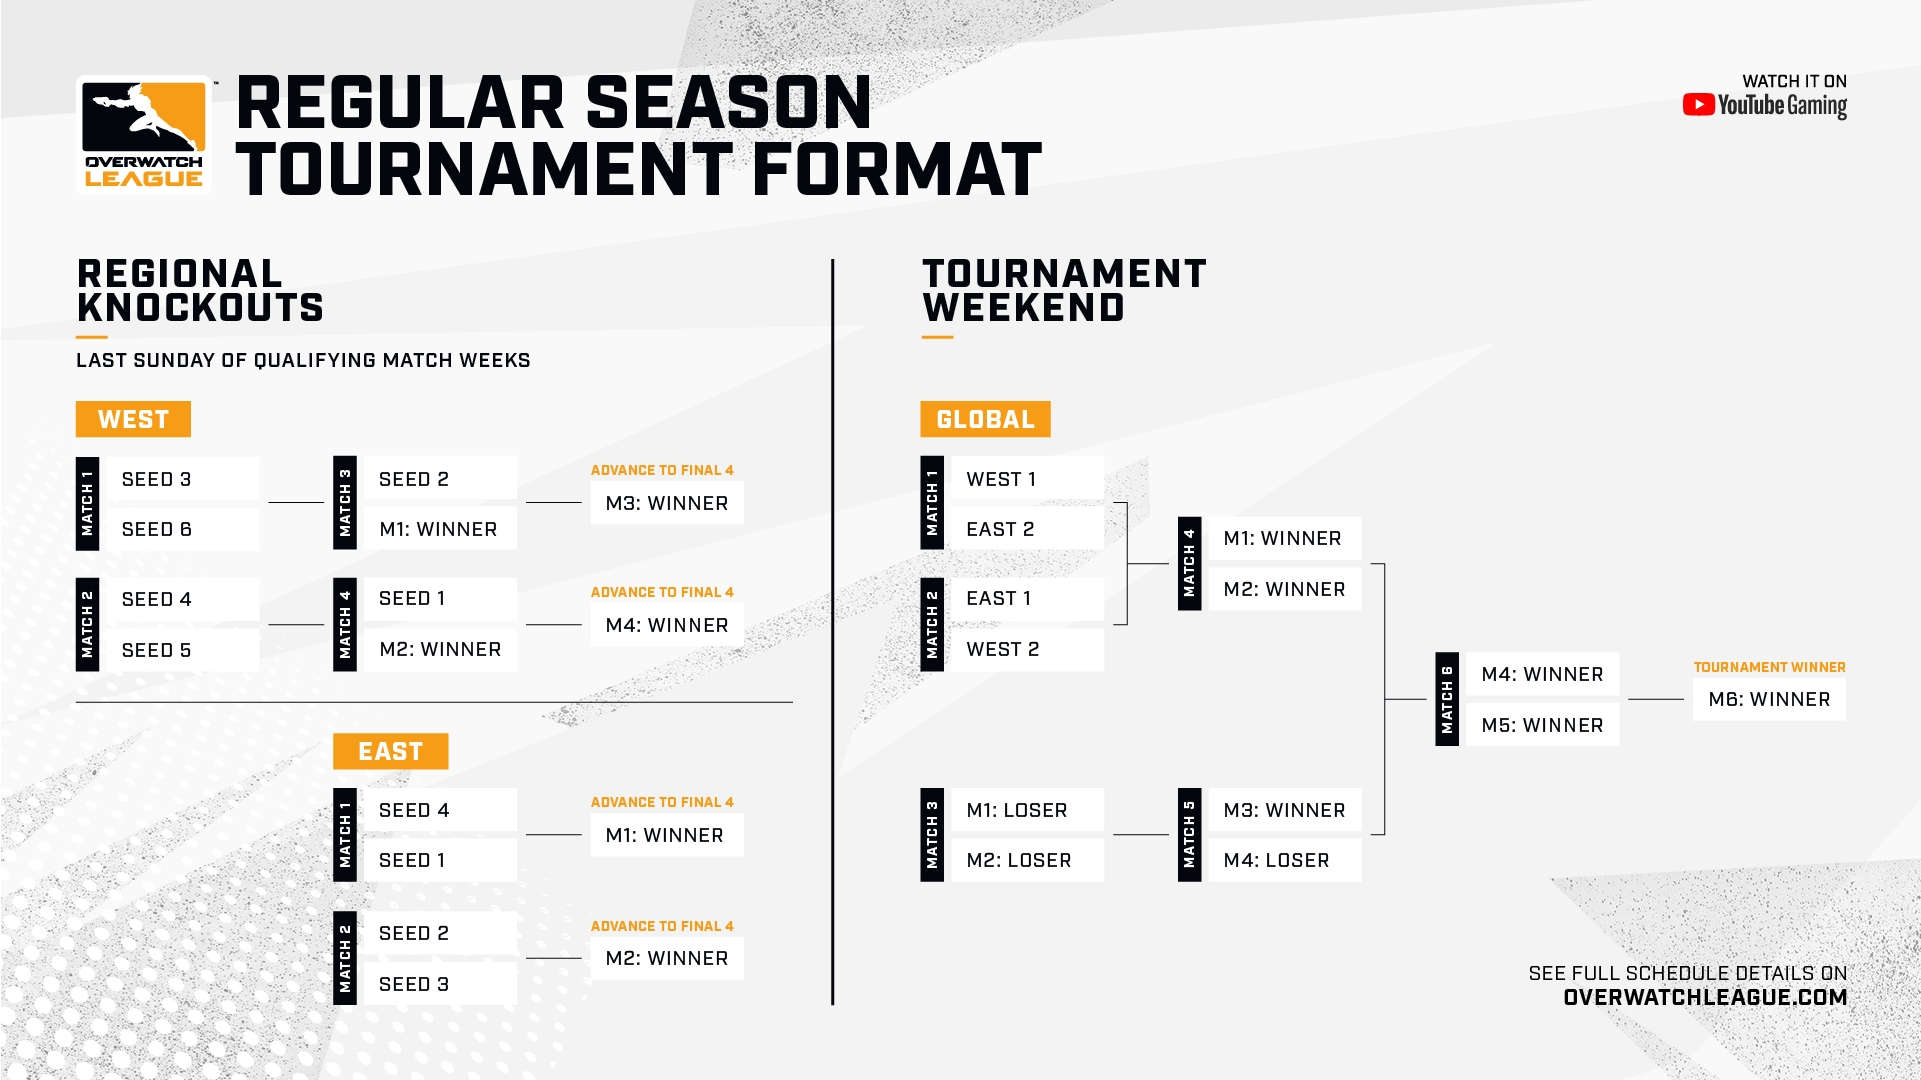
\includegraphics[width=\textwidth]{images/owl-tournament-format.png}
    \caption{OWL 2021 Tournament Format}
    \label{fig:owl-tournament-format}
\end{figure}

Regional knockouts are single elimination.
\begin{itemize}
    \item Round 1: (west) match 1, 2; (east) match 1, 2
    \item Round 2: (west) match 3, 4
\end{itemize}

Global finals are double elimination.
\begin{itemize}
    \item Round 3: (global) match 1, 2
    \item Round 4: (global) match 3, 4
    \item Round 5: (global) match 5
    \item Round 6: (global) match 6 - the tournament final
\end{itemize}

In fact, this description of tournament is so powerful that when we let every round to include only one match, we can implement general skill-rating algorithms such as Elo Rating.

\section{API Design}
\label{as:matchmaking-api_design}

\subsection{Overview}
\label{as:matchmaking-api_design-overview}
Now that we have a powerful abstraction of tournaments, we are ready to describe the API design. In specific, a complete tournament consists of the following steps:
\begin{enumerate}
    \item \texttt{GET /api/v1/tasks/<task\_pk>/start\_matchmaking} with parameters:
    \begin{itemize}
        \item List of submission IDs
        \item Matchmaker type (e.g., round-robin)
    \end{itemize}
    \item A \texttt{MatchmakingSession} object is created and stored in DB
    \item \texttt{kickstart} method of the \texttt{MatchmakingSession}'s \texttt{Matchmaker} is called. We get a list of \texttt{MatchParticipant}s and \texttt{Match}es. We store the \texttt{MatchParticipant}s and schedule the \texttt{Match}es just like scheduling single-agent evaluation jobs.
    \item Every call to \texttt{submit\_job} RESTful API will trigger a signal\footnote{Signal is a trigger mechanism in Django. For more details, please check \href{https://docs.djangoproject.com/en/4.0/topics/signals/}{https://docs.djangoproject.com/en/4.0/topics/signals/}} to check if the job has a corresponding \texttt{MatchmakingSession}\footnote{For backward compatibility (i.e., supporting evaluation jobs that is not part of any tournament), we allow a \texttt{Job} to have no corresponding \texttt{MatchmakingSession}.}:
    \begin{enumerate}
        \item If yes, check if all \texttt{pending\_jobs} in the \texttt{MatchmakingSession} are finished
        \item If also yes, call \texttt{schedule} method of the \texttt{MatchmakingSession}'s \texttt{Matchmaker} instance
        \begin{enumerate}
            \item Schedule the returned matches by creating \texttt{Job}s if necessary - at the same time reset \texttt{pending\_jobs} of the \texttt{MatchmakingSession}
            \item Update the ratings of the \texttt{MatchParticipant}s using the return value
            \item If concluded, set \texttt{ongoing} of the \texttt{MatchmakingSession} to \texttt{False}
        \end{enumerate}
    \end{enumerate}
\end{enumerate}

\subsection{Models}
There are two new models required for multi-agent matchmaking: \texttt{MatchParticipant}, \texttt{MatchmakingSession}. In addition, we need a \texttt{Match} wrapper class to represent the list of participants involved in a match. However, unlike the other two models that need to be stored in the database, \texttt{Match} is temporary. The concrete implementation of these models is shown in Code~\ref{code:multi-agent-models}.

\begin{code}
\begin{minted}[frame=lines,framesep=2mm,baselinestretch=1.2,bgcolor=LightGray,fontsize=\footnotesize,linenos,breaklines,samepage]{python}
from django.db import models

class MatchParticipant(models.Model):
    submission = models.ForeignKeyField(Submission)
    rating = models.FloatField()
    

class MatchmakingSession(models.Model):
    participants = models.ManyToManyField(MatchParticipant)
    pending_jobs = models.ManyToManyField(Job)
    ongoing = models.BooleanField()

class Match():
"""
Match is a list of submission IDs corresponding to the participants of this match.
"""
    def __init__(self, ids: List[int]):
        self.ids = ids
\end{minted}
\captionof{listing}{Multi-agent Matchmaking Models}
\label{code:multi-agent-models}
\end{code}

\subsection{Changes to Existing Models}
\begin{enumerate}
    \item \texttt{Job} model needs to support more than one related \texttt{Submission}s - this can be easily achieved by changing \texttt{ForeignKeyField} to a \texttt{ManyToManyField}.
    \item \texttt{Job} needs to bind to a \texttt{MatchmakingSession} so that when the \texttt{Job} is submitted, the \texttt{Matchmaker} can be notified. One possible way:\\ \texttt{matchmaking\_session = models.ForeignKeyField(MatchmakingSession, null=True)}
\end{enumerate}

\subsection{Matchmaking Logic Abstraction}
\label{as:matchmaking-api_design-matchmaking_logic_abstraction}
As shown in Section~\ref{as:matchmaking-api_design-overview}, the decision-making of the entire matchmaking process is abstracted as the \texttt{kickstart} and \texttt{schedule} method of a \texttt{Matchmaker}. This is exactly where the tournament rules and/or matchmaking algorithm should be implemented. Below is an abstract base class for \texttt{Matchmaker}:

\begin{code}
\begin{minted}[frame=lines,framesep=2mm,baselinestretch=1.2,bgcolor=LightGray,fontsize=\footnotesize,linenos,breaklines,samepage]{python}
class BaseMatchmaker():
"""
Matchmaker class must be stateless - every time a new instance of Matchmaker will be created.
"""
    def kickstart(self, participants: List[MatchParticipant]) -> (List[MatchParticipant], List[Match]):
        pass

    def schedule(self, participants: List[MatchParticipant], jobs: List[Job]) -> (bool, List[MatchParticipant], List[Match]):
        pass
\end{minted}
\captionof{listing}{\texttt{Matchmaker} Abstract Base Class}
\label{code:matchmaker-abc}
\end{code}

Explanation of input parameters:
\begin{itemize}
    \item Pool of participants - in our case, each participant has
    \begin{itemize}
        \item Submission ID
        \item Current rating/score
    \end{itemize}
    \item Match history, in particular, every match should at least have
    \begin{itemize}
        \item IDs of all participating submissions
        \item Outcome of the match
    \end{itemize}
\end{itemize}

Explanation of the outputs:
\begin{itemize}
    \item Whether this tournament has concluded or not
    \item List of updated rating/score for all submissions
    \item List of scheduled matches (if the tournament hasn't concluded yet)
\end{itemize}
